\documentclass{article}
\usepackage{amsmath}
\usepackage{amsfonts}
\usepackage{amssymb}
\usepackage{mathrsfs}
\usepackage{dsfont}
\usepackage{cancel}

\usepackage{graphicx}


\setlength\parindent{0pt}

\author{Pranav Tikkawar}
\title{Chapter 2 }

\begin{document}
\maketitle
\section*{2.1 Wave Equation}
$$ u_{tt} = c^2 u_{xx}, x \in \mathds{R} ***$$
\textbf{Theorem 1: d'Alembert}\\
Any solution to *** is of form $$ u(x,t) = f(x + ct) + g(x - ct) $$  where $f$ and $g$ are twice differentiable functions.\\
\textbf{Proof:} Method 1\\
$$ (d_t^2 - c^2 d_x^2 )u  = 0 $$
$$ (d_t - c d_x)(d_t + c d_x)u = 0 $$
Let $ v = (d_t + c d_x)u $\\
Then $ (d_t - c d_x)v = 0 $
This is a transport equation. The general solution is $$ v(x,t) = h(x + ct) $$ for some function $h$.\\
$$ u_t + c u_x  = h(x + ct) $$
Inhomogeneous transport equation.\\
We can use linearity to find the general solution. Since it will be the sum of homogenous plus another function\\
$$ u = u_p + g(x-ct) $$
Where $u_p$ is a particular solution.\\
$$ u_p = h(x + ct) $$
$$h'c + ch' =  f$$ 
$$h' = \frac{f}{2c}$$
$$ u = \frac{1}{2c} \int f(x + ct) dx + g(x - ct)$$***

$$(\partial_t - c \partial_x)(\partial_t + c \partial_x)u = 0 $$
$$ f(x+ct), g(x-ct)$$
Recall that $f(x+ct)$ is a wave traveling left at speed c and $g(x-ct)$ is a wave traveling right at speed c\\
Thus the solution is a wave traveling with speed c in both directions.\\
The wave equation is bidirectional.(unlike the transport equation)\\
\textbf{Remark:} u is a superposition of two waves traveling in opposite directions at fixed speed c.\\
\textbf{Method 2:} \\
Characteristic variable: 
$$ \xi = x + ct, \eta = x - ct $$
Then we can write 
$$ u(x,t) = u(\xi(x,t),\eta(x,t)) $$
$$ \partial_x = \partial_\xi + \partial_\eta $$
$$ \partial_t = c \partial_\eta - c \partial_\xi $$
Factoring gives us 
$$ \partial_t^2 - c^2 \partial_x^2 = (\partial_t -c\partial_x)(\partial_t + c \partial_x) $$
Plugging in we get 
$$ -2c\partial_\eta \cdot 2c \partial_\xi  $$
$$ -4c^2 \partial_\xi \partial_\eta = 0 $$ 
Thus we can differentiate with respect to $\xi$ and $\eta$ to get the general solution.
$$ u_{\xi \eta} = 0 $$
Integrating gives us
$$ u = f(\xi) + g(\eta) $$
\textbf{Theorem 2: (d'Alembert 1747)}
$$\begin{cases}
    u_{tt} = c^2 u_{xx}, t>0, x \in \mathds{R}\\
    u(x,0) = \phi(x), x \in \mathds{R}\\
    u_t(x,0) = \psi(x), x \in \mathds{R}
\end{cases} 
$$
Where $\phi$ is initial displacement and $\psi$ is initial velocity.\\
$$ u(x,t) = \frac{1}{2} \left( \phi(x + ct) + \phi(x - ct) \right) + \frac{1}{2c} \int_{x - ct}^{x + ct} \psi(s) ds $$
\textbf{Proof:} By theorum 1: 
$$ u(x,t) = f(x+ct) + g(x-ct)$$
Find f,g using ICs 
$$ u(x,0) = f(x) + g(x) = \phi(x) $$
$$ u_t(x,t) = cf'(x+ct) - cg'(x-ct) $$
$$ u_t(x,0) = c f'(x) - c g'(x) = \psi(x) $$
$$\begin{cases}
    c f' + cg' = c \phi'\\
    c f' - cg' = \psi
\end{cases}
$$
Adding gives us
$$\begin{cases}
    2cf' = c \phi' + \psi\\
    2cg' = c \phi' - \psi
\end{cases}
$$
$$
\begin{cases}
    f' = \frac{1}{2} \left( \phi' + \frac{\psi}{c} \right)\\
    g' = \frac{1}{2} \left( \phi' - \frac{\psi}{c} \right)
\end{cases}
$$
$$f(s) = \frac{1}{2} \phi(s) + \frac{1}{2c} \int_0^s \psi(y) dy + A$$
$$g(s) = \frac{1}{2} \phi(s) - \frac{1}{2c} \int_0^s \psi(y) dy + B$$
$$
\begin{cases}
    f(0) = \frac{1}{2} \phi(0) + A\\
    g(0) = \frac{1}{2} \phi(0) + B
\end{cases}
$$
$$
f(0) + g(0) = \phi(0) + A + B
$$
$f+g = \phi$ which cancels outs\\
Thus we can set $A + B= 0 $\\
\begin{align*}
    u(x,t) &= f(\xi) + g(\eta)\\
    &= \frac{1}{2}\phi(\xi) + \frac{1}{2c} \int_0^\xi \psi(y) dy + A \\
    &+ \frac{1}{2}\phi(\eta) - \frac{1}{2c} \int_0^\eta \psi(y) dy + B
\end{align*}
\begin{align*}
    u(x,t) &= f(\xi) + g(\eta)\\
    &= \frac{1}{2}\phi(\xi) + \frac{1}{2c} \int_0^\xi \psi(y) dy  \\
    &+ \frac{1}{2}\phi(\eta) - \frac{1}{2c} \int_0^\eta \psi(y) dy\\
    &= \frac{\phi(\xi) + \psi(\eta)}{2} + \frac{1}{2c} \left( \int_0^\xi \psi(y) dy - \int_0^\eta \psi(y) dy \right)\\
    &= \frac{\phi(\xi) + \psi(\eta)}{2} + \frac{1}{2c} \int_{\eta}^{\xi} \psi(y) dy
\end{align*}
2 families of characteristics lines:\\
$$ x \pm ct = constant$$
On one of these lines they are constant.\\
\textbf{Example 1: }\\
$\psi(x) = 0$\\
$$ u(x,t) = \frac{1}{2} \left( \phi(x + ct) + \phi(x - ct) \right)$$
Initial displacement $\phi$ splits into two parts. Each with half the amplitude. and one is opposite direction from the other\\
\textbf{Example 2: }\\
$\psi(x) = 0$\\
Interaction of "pulse".\\
They constructively interfere and they keep their shape.\\
\textbf{Example 3: }\\
$\phi(x) = 0$\\
$$ u(x,t) = \frac{1}{2c} \int_{x - ct}^{x + ct} \psi(y) dy$$
If x is too large of magnititue it will be zero.\\
As we increase t, the integral will increase.\\
For largers t, I have more choses of x that make u nonzero.\\
\textbf{Example 4: }\\
$\psi(x) = 0, \phi(s) = sin(s)$
$$ u(x,t) = \frac{1}{2} \left( sin(x + ct) + sin(x - ct) \right)$$
$$ u(x,t) = sin(x) cos(ct)$$
This is a standing wave! 
\textbf{Remark 1:}\\
If $\psi = 0$ and $\phi$ is localized then the right and left moving waves will (in the long run) always separate.\\
If $\phi$ is not localized then then they don't separate
\textbf{Remark 2:} $\phi = 0 $ and $\psi$ is localized, fix $x_0$ then $u(x_0,t) = 0 $ for all $t >t_0$.\\
The intial disturbance is felt at $x_0$ and then the affect will be gone
\section*{2.2 Causality and Energy }
$$\begin{cases}
    u_{tt} = c^2 u_{xx} \\
    u(x,0) = \phi(x)\\
    u_t(x,0) = \psi(x)
\end{cases}
$$
D'Alembert solution:
$$ u(x,t) = \frac{1}{2} \left( \phi(x + ct) + \phi(x - ct) \right) + \frac{1}{2c} \int_{x - ct}^{x + ct} \psi(s) ds $$
\textbf{Lemma: }
If $\phi$ and $\psi$ are compactly supported in $[a,b]$, (this means outside the interval they are zero) then $u(x,t) = 0$ outside of $R$ where R is the "domain of influence of the interval $[a,b]$\\
The boundary lines are $x - ct =b$ and $x + ct = a$\\
This is like an open cone.\\
$$ R = \text{ regieon where distubances are felt}$$
\textbf{Proof:}\\
By assumption $\phi(s)$ and $\psi(s)$ are zero for $s < a $\\
Thus the outside area is $x + ct < a$\\
Also $x - ct \leq x+ct < a$\\
In that region $u(x,t) = 0$\\
Similarly we can do this for the region $x - ct > b$\\
Thus we can conclude that $u(x,t) = 0$ outside of the region $R$. Due to the fact that both $\phi =0$ and the integral $\int_{x-ct}^{x+ct} \psi(s) ds = 0$ \\

In the limiting case. This is a "light cone"\\
This is where we have $x_0$ being the point of disturbance.\\
The region of influence is the area where the disturbance is felt.\\ 
$$ x +ct = x_0, x - ct = x_0$$
$$ x \pm ct = x_0$$

$ \phi(x_0)$ and $\psi(x_0)$ affect the values of $u(x,t)$ if $x \pm ct = x_0$ or $x_0 \in [x - ct, x + ct]$\\

\textbf{Reverse Questions:}\\
Fix value of u and see what initial conditions affect this.\\
We need initial values at $x_0 \pm ct_0$ and in $[x_0 - ct_0, x_0 + ct_0]$\\
This is like a triangle\\
This is called the interval/region of dependance of the point $x_0$.\\
\textbf{Remark: }\\
$$u(x_0,t_0) = \frac{1}{2} \left( \phi(a) + \phi(b) \right) + \frac{1}{2c} \int_{a}^{b} \psi(s) ds$$
$$b-a = 2ct_0$$
$$ u(x_0,t_0) = \frac{1}{2} \left( \phi(a) + \phi(b) \right) + t_0 \cdot \frac{1}{b-a} \int_{a}^{b} \psi(s) ds$$
Note that the first term is average displacement and the second term is average velocity.\\
\textbf{Example: }\\
$$\psi = 0, \phi = \begin{cases}
    1, & x \in [0,1]\\
    0, & \text{otherwise}
\end{cases}
$$
say $c =1 $\\
Now: add image of the region of influence.\\
\begin{center}
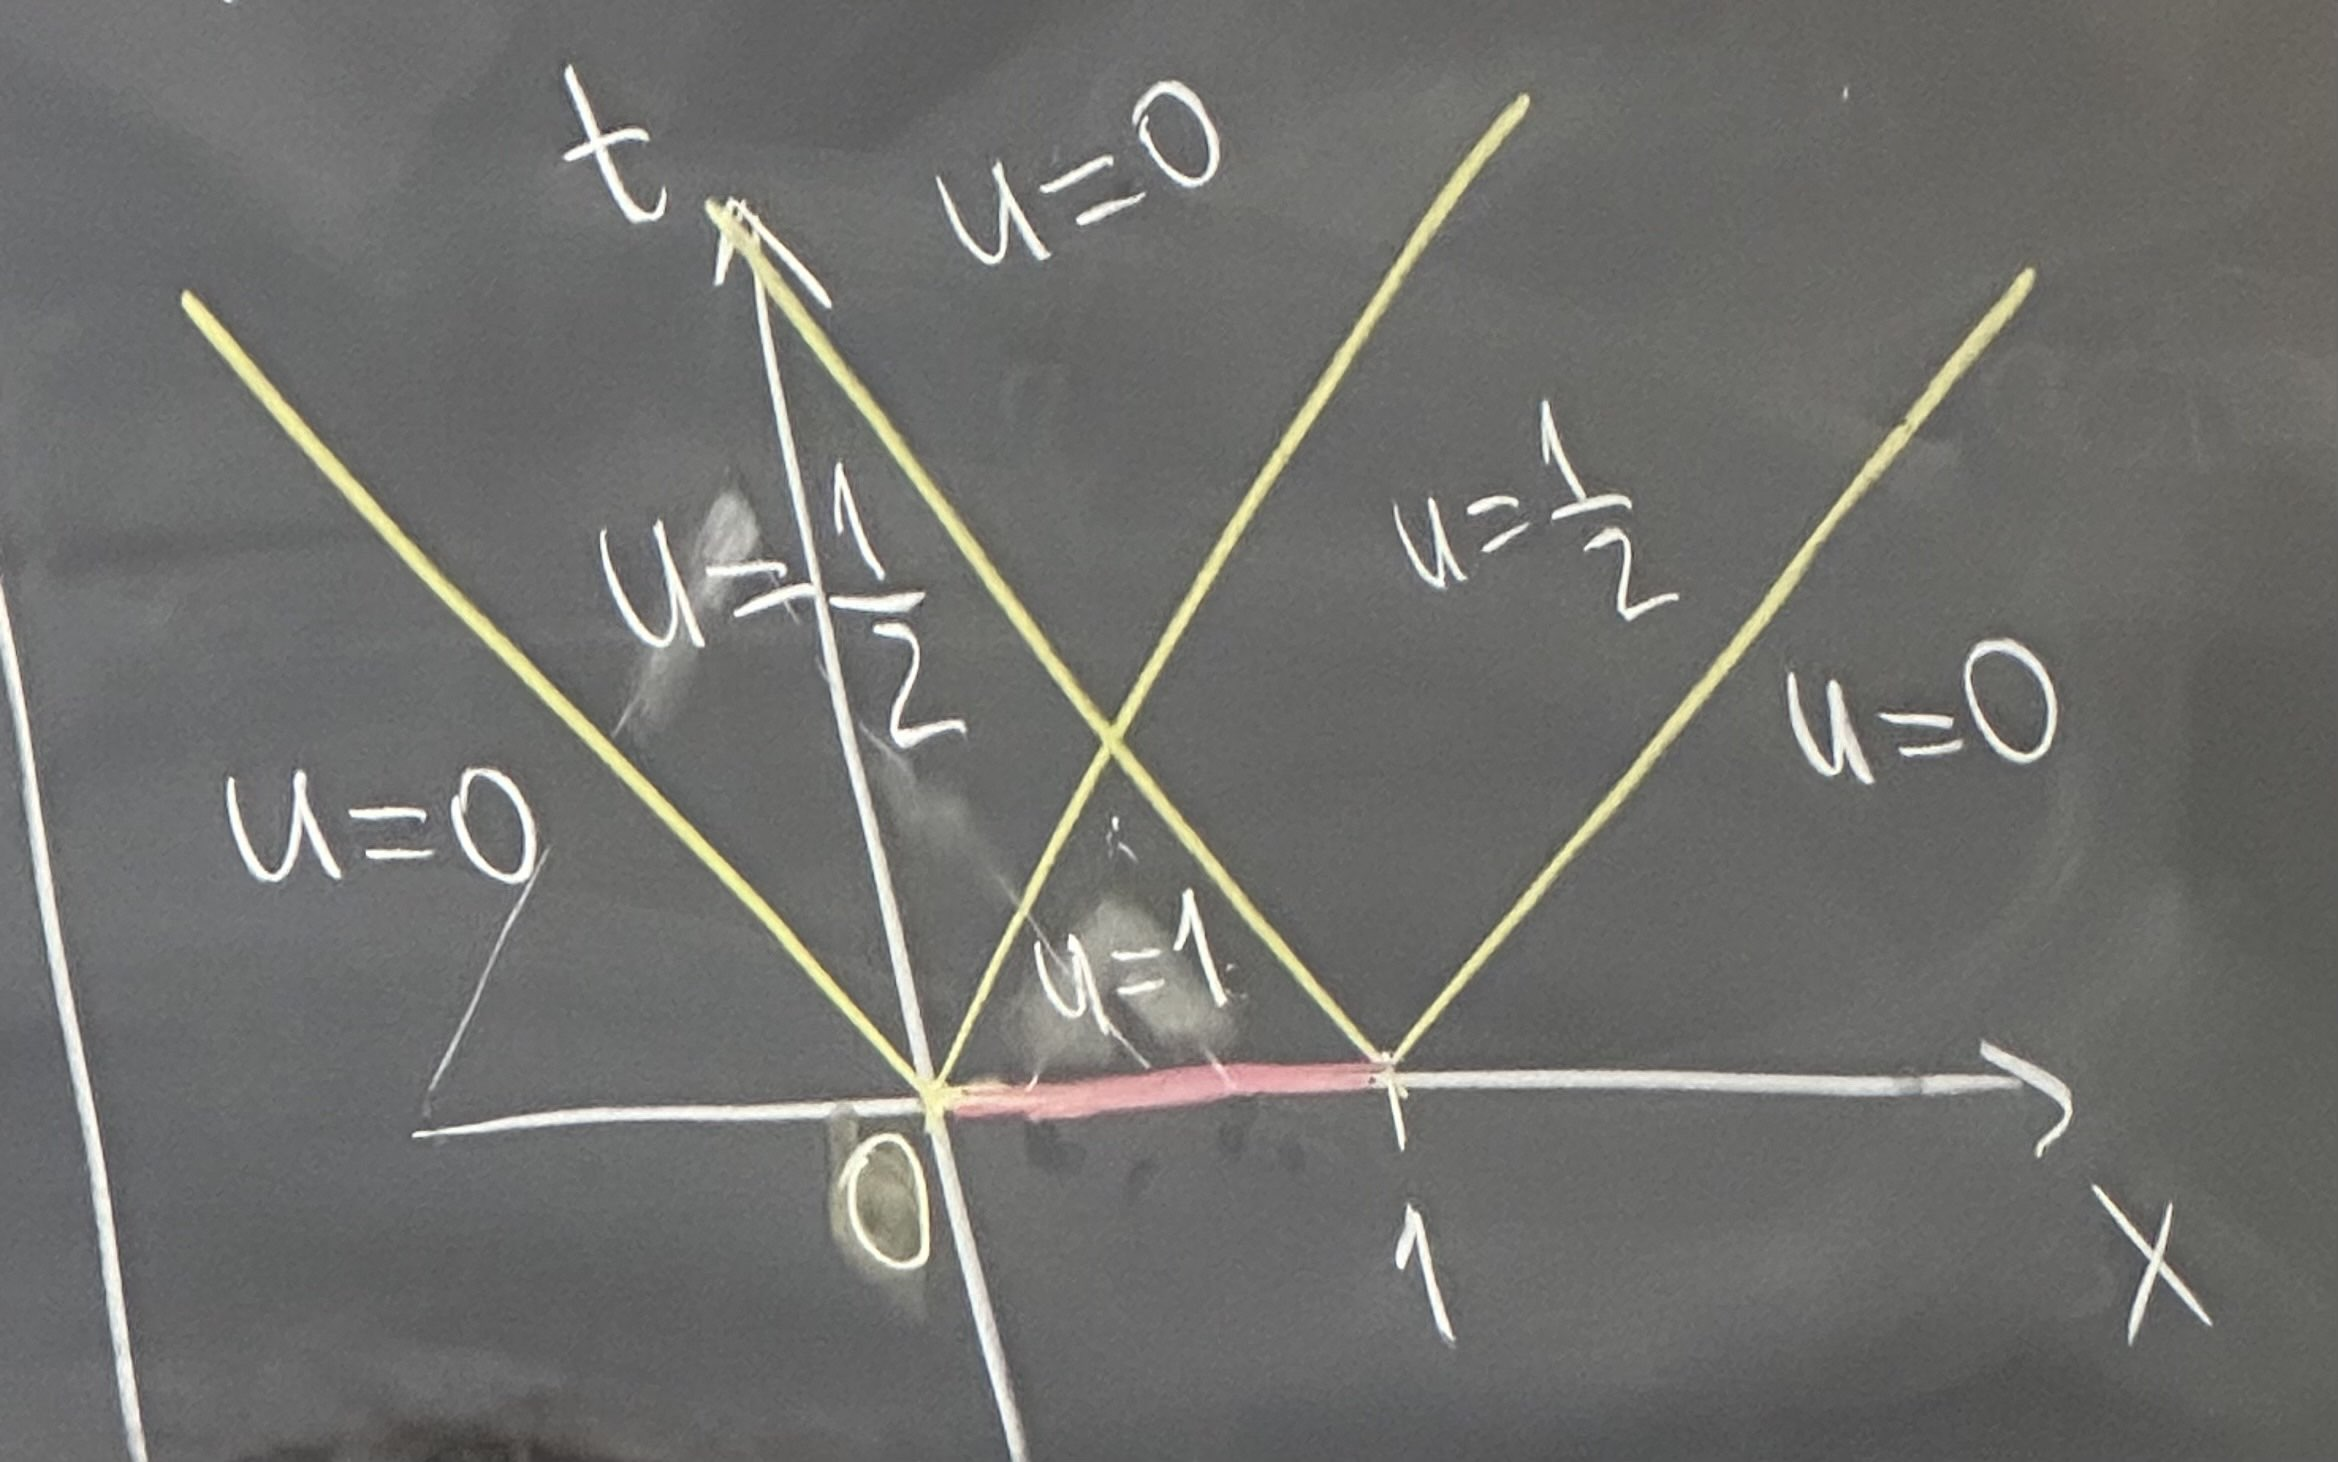
\includegraphics[width=0.5\textwidth]{IMGs/PDEs_Triangle.jpg}
\end{center}
We can view this as two Vs that intersect at a point and then separate.\\
Outside the two Vs it is 0, inside both it is 1, inside one it is 1/2\\
And if it is in the middle it is also 0\\
\textbf{Finite speed of propagation:}\\
Localized initial data ie compactly supported. (0 outside some interval)\\
This implies that $u(x,t)$ is also localize for any $t>0$.\\
If $\phi, \psi$ are supported in $[a,b]$ then $u(x,t)$ is supported in $[a-ct,b+ct]$\\
when you are at position $x$ you would feel the disturbance at time $t \geq \frac{x-b}{c}$ or distance from $x$ to the interval

\textbf{Remark:} \\
The wave equation has no smoothing effect.\\
Singularity and discontinuities remain \\
Non-smooth initial data does not become smooth at any time.\\
Say $\phi$ has a discontinuity/ singularuty at $x_0$, then $u(x,t)$ is singular whenever $x \pm ct = x_0$\\
Singularity propogrates along characteristics.\\

\textbf{Causality: }\\
Causality means the effect comes after the cause.\\
Cause = distubance at $x_0$\\
Effect = disturbance at other points\\
Since there is a finite speed of propagation, the disturbance at $x_0$ can only affect points in the region of influence.\\

\textbf{Huygen's Principle:} \\
The disturbance in $[a,b]$ reaches $x_1$ at time $t_1$ and then it remains in the region of influence for all $t > t_1$.\\
If $\psi = 0$ region of influence of $[a,b]$ is just the effect is felt only at time $t_1$ and no lingering effects. In other words, just feel once then gone.\\
\textbf{Kirkchoff's formula}\\
In 3d the solution to the wave equation is given by Kirkchoff's formula.\\
it only uses $\phi$ and $\psi$ on the boundary of the region of influence.\\
this is true for $n \geq 3$ and odd dimensions.\\
So in 2D this is not true! \\

\textbf{Energy Conservation:}\\
$$ u_{tt} = c^2 u_{xx}$$
$$ E(t) = \frac{1}{2} \int_{\mathds{R}}u_t^2(t,x) + c^2 u_x^2(t,x) dx$$
Then $E(t)$ is constant in time. In particular $E(t) = E(0)$\\
\textbf{Remark:} \\
$\phi, \psi$ are localized, in other words, vanish outside of some interval. $[a,b]$\\
Thus the function $u(x,t)$ is also localized in $[a-ct,b+ct]$\\
\textbf{Proof:}\\
$$ E'(t) = \int_{\mathds{R}} u_t u_{tt} + c^2 u_x u_{xt} dx$$
$$ E'(t) = \int_{\mathds{R}} u_t c^2 u_{xx} + c^2 u_x u_{xt} dx$$
This motivates integrating by parts.\\
$$ \int_{\mathds{R}} u_x u_{tx} dx = \left[ u_x u_t \right]_{-\infty}^{\infty} - \int_{\mathds{R}} u_{xx} u_t dx$$
$$ E'(t) = \int_{\mathds{R}} u_t c^2 u_{xx} - c^2 u_{xx} u_t dx = 0$$
\textbf{Remark:} \\
In higher dimensions $u_x^2$ is replaced by $|\nabla u|^2$\\

\subsection{2.3: Heat Equation}
$$ u_t = k u_{xx}$$
Now we consider this on a finite interval \\
$$t \in (0,T), x \in (0,L)$$
$$ R = (0,T) \times (0,L)$$
$$ \bar{R} = [0,T] \times [0,L]$$
This is inculding the boundary.\\
We also was all boundary without the top "t" side call it $\Gamma$\\
This is called the parabolic boundary.\\
\textbf{Max Principle:}\\
If $u(x,t)$ is a solution to the heat equation in $R$ and it is continuous on $\bar{R}$ 
Then $max(u)_{\bar{R}} = max(u)_{\Gamma}$\\
This is an extension of the extreme value theorem\\
\textbf{Proof:}\\
$$v(t,x) = u(t,x) + \epsilon x^2$$
Where $\epsilon > 0$\\
$$v_t = u_t = k u_{xx} = k( v_{xx} - 2\epsilon)$$
$$v_{xx} = u_{xx} + 2\epsilon$$
Thus we gain:
$$ v_t = k v_{xx} - 2k\epsilon$$
$$ v_t < k v_{xx}$$
$v$ attains its maximum on the boundary.\\
Let $v(t_0,x_0) = max(V)_{\bar{R}}$
if $(t_0,x_0) \in \bar{R}$ then $v_t \leq k v_{xx}$\\
$$ v(t_0,x_0) = 0 $$
$$ f(x) = v(t_0,x) \text{ has max at } x_0 \text{, then}$$
$$ f''(x) = 0 $$
$$ v_t(t_0,x_0) < k v_{xx}(t_0,x_0) \leq 0$$
This is contradiction.\\
if $(t_0,x_0) \in $ top boundary ie $t_0 = T, x \in (0,L)$\\
$$ g(t) = v(t,x_0) $$
has max at $T$ then $g'(T) \geq 0$\\
$$ g'(T) = v_t(T,x_0) = u_t(T,x_0) \leq 0$$
$$ 0 \geq v_t < k v_{xx} \geq 0$$
This is a contradiction.\\
\textbf{Consider} \\
Why does it work on gamma?\\
Thus $max(v)_\Gamma = max(v)_{\bar{R}}$\\

Now we need to prove this for $u$\\
Let $M = max(u)_{\Gamma}$\\
goal: $u(t,x) \leq M$ for all $(t,x) \in \bar{R}$\\
\begin{align*}
    u + \epsilon x^2 &= V\\
    & \leq max(V)_{\Gamma} \\
    & = max(u + \epsilon x^2)_{\Gamma}\\
    & \leq max(u)_{\Gamma} + \epsilon L^2
\end{align*}
Let $\epsilon \to 0$\\
$$ u \leq max(u)_{\Gamma}$$
\textbf{Remark:} \\
Strong max principle says that $max(u)_{\bar{R}}$ can \textbf{only} be attained on $\Gamma$\\
Immediate consequence of this the solution to the heat equation is unique.\\
\textbf{Corollary:} \\
We can do this for minimum as well.\\
\textbf{Proof:} \\
Let $v = -u$\\
Then $v_t = -u_t = -k u_{xx} = k v_{xx}$\\
Then we can apply the max principle to $v$\\
\textbf{Theorem: Uniqueness} \\
The solution to the heat equation is unique.\\
\textbf{Proof:} \\
$$\begin{cases}
    u_t = k u_{xx} + f(t,x)\\
    u = u_0 
\end{cases}
$$
The following are the intital/boundary conditions.\\
$$\begin{cases}
    u(t,0) = a(t)\\
    u(t,L) = b(t)\\
    u(0,x) = \phi(x)
\end{cases}
$$
This has at most one solution.\\
\textbf{Proof:} \\
Suppose $u_1, u_2$ are two solutions.\\
Let $w = u_1 - u_2$\\
Then $w_t = k w_{xx}$\\
$$\begin{cases}
    w(t,0) = 0\\
    w(t,L) = 0\\
    w(0,x) = 0
\end{cases}
$$
$$ max(w)_{\bar{R}} = 0$$
$$ min(w)_{\bar{R}} = 0$$
Thus $w = 0$ ie $u_1 = u_2 $ in $R$ \\
\textbf{Remark:} \\
We cant prescribe data for $u$ on top boundary. It is determned by the PDE and the initial data.\\
\textbf{Proof 2:} \\
$$E(t) = \int_0^L w^2(t,x) dx$$
$$E'(t) = 2 \int_0^L w w_t dx = 2 \int_0^L w k w_{xx} dx $$
$$ = 2k \left[ w w_x \right]_0^L - 2k \int_0^L w_x^2 dx$$
$w = 0$ on the boundary.\\
$$ = -2k \int_0^L w_x^2 dx \leq 0$$
$$ E'(t) \leq 0$$
ie heat dissipates over time.\\
$$E(t) \leq E(0)$$
$$\int_0^L w^2(0,x) dx = 0$$
Since we know that by our definition of the integral it is non negative.\\
Thus $0 \geq w^2(0,x) \geq 0$\\
Thus $w = 0$\\
Thus $u_1 = u_2$\\
\textbf{Remark:} \\
The heat equation is a smoothing effect.\\
$$u_{xx}(A) < 0 \implies u_{t}(A) < 0$$
Peaks go down and valleys go up.\\
Want to reach equilibrium.\\
\textbf{Remark:} \\
Uniqueness for heat IBVP holds in: \\
\textbf{Stability estimates:} \\
\textbf{Lemma 1:} \\
Consider $R$ and $\Gamma$
$$\begin{cases}
    u_t = ku_{xx}, \in R\\
    u = u_0 \in \Gamma
\end{cases}
$$
$$max(u)_{\bar{R}} = max(u)_{\Gamma}$$
\textbf{Proof:} \\
$$-|u_0| \leq u_0 \leq |u_0|$$
$$ u \leq max(u)_{\bar{R}} = max(u)_{\Gamma} \leq max(|u|)_\Gamma$$
$$ -u \geq min(u)_{\bar{R}} = min(u)_{\Gamma} \geq -max(|u|)_\Gamma$$
$$ |u| \leq max(|u|)_\Gamma \text{ everywhere}$$
Initial/boundary data $u_0$ controls $u$ everywhere.\\
\textbf{Corollary:} \\
$$\begin{cases}
    \partial_t u_1 = k \partial_{xx} u_1
    u_1(x,0) = \phi_1(x)\\
    u_1(0,t) = u_1(l,t) =  0
\end{cases}$$
$$\begin{cases}
    \partial_t u_2 = k \partial_{xx} u_2
    u_2(x,0) = \phi_2(x)\\
    u_2(0,t) = u_2(l,t) =  0
\end{cases}$$
We think $u_1$ as the true one and the $u_2$ is the experimentally derived one with perturbations.\\
$$ max |u_2 - u_1|_{\bar{R}} \leq max|\phi_2 - \phi_1|_{[0,l]}$$
\textbf{Proof:} \\
Let $u = u_2 - u_1$\\
Let $\phi = \phi_2 - \phi_1$\\
$u$ will solve the heat equation with initial condition $\phi$\\
$$\begin{cases}
    u_t = k u_{xx}\\
    u(x,0) = \phi(x)\\
    u(0,t) = u(l,t) = 0
\end{cases}
$$

By lemma 1 we have that $max(u)_{\bar{R}} \leq max(u)_{[0,l]}$\\

\textbf{Lemma 2:} \\
$$ \int_{0}^{l} u^2 dx \leq \int_{0}^{l} \phi^2 dx$$
$$
\begin{cases}
    u_t = k u_{xx}\\
    u(x,0) = \phi(x)\\
    u(0,t) = u(l,t) = 0
\end{cases}
$$
\textbf{Proof:} \\
$$ E(t) = \int_{0}^{l} u^2 dx$$
$$ E'(t) \geq 0 \implies E(t) \leq E(0)$$
\textbf{Corollary 2:} \\
In the setting of Corollary 1:\\
$$ \int_0^l |u_2 - u_1|^2 dx \leq \int_0^l |\phi_2 - \phi_1|^2 dx$$
$f = f(x)$ on I\\
$$||f||_\infty = max|f|_I$$
$$||f||_\infty = 0 \implies f = 0$$\\
$$||f||_{L^2} = \left( \int_I |f|^2 dx \right)^{1/2}$$
This is known as the $L^2$ norm; mean-squared\\
$$|f(x)| \leq ||f(x)||_\infty$$\\
$|f(x)|^2 \leq ||f(x)||_\infty^2$\\
$$\int_I |f(x)|^2 dx \leq ||f(x)||_\infty^2 \int_I dx$$
$$||f||_{L^2} \leq ||f||_\infty \sqrt{|I|}$$

$$||u_2(\star, t) - u_1(\star, t)||_{L^2} \leq ||\phi_2 - \phi_1||_{L^2}$$
The size at any time is controlled by the intial data.\\

\section*{2.4: Heat Equation on the Real Line}
\textbf{Theorem:} \\
$$S(x,t) = \frac{1}{\sqrt{4\pi kt}} e^{-\frac{x^2}{4kt}}$$
This is the fundamental solution to the heat equation.\\
\begin{enumerate}
    \item $S_t =  S_{xx}$
    \item $\int_{-\infty}^{\infty} S(x,t) dx = 1, \forall t > 0$
    \item $\lim_{t \to 0^+} \int_{R} S(x,t) f(x) dx = f(0)$ for all continuous and bounded $f$ on $\mathds{R}$
\end{enumerate}
$\lim_{t \to 0^+} S(x,t) = \begin{cases}
        \infty, & x = 0\\
        0, & x \neq 0
\end{cases}$
\textbf{Proof:} \\
Need to prove:\\
$$ \lim_{t \rightarrow 0^+}\int_R S(x,t) [f(x) - f(0)] dx = 0$$
Fix $\epsilon > 0$ then there exists $\delta > 0$ such that $|f(x) - f(0)| < \epsilon$ for $|x-0| < \delta$\\
$$ I = \int_{|x| < \delta} + \int_{|x| \geq \delta}$$
$$ |I_1| \leq \int S(x,t) |f(x) - f(0)| dx$$
$$ |f(x) - f(0)| < \epsilon$$
$$ |I_1| \leq \epsilon \int_{x \leq \delta} S(x,t) dx \leq \epsilon $$
This works for any $t$\\
$$ |f(x)| \leq M $$
$$ |f(x) - f(0)| \leq 2M$$
$$ |I_2| \leq 2M \int_{|x| \geq \delta} S(x,t) dx$$
Let $y = \frac{x}{\sqrt{4t}}$\\
Then $y^2 = \frac{x^2}{4t}$\\
$$ |I_2| \leq 2M \int_{|y| \geq \frac{\delta}{\sqrt{4t}}} \frac{1}{\sqrt{4\pi t}} e^{-y^2} \sqrt{4t} dy$$
$$ |I_2| \leq \frac{2M}{\sqrt{\pi}}\int_{|y| \geq \frac{\delta}{\sqrt{4t}}} e^{-y^2} dy$$
Notice that the integral goes to 0 as $t \to 0$\\
$$ \int_{R} g(y) dy = \lim_{a \rightarrow \infty}\int_{-c}^{c} g(y) dy$$
$$ \int_{R} g(y) dy = \lim_{t \rightarrow 0^+} \int_{-1/t}^{1/t} g(y) dy$$
$$ \int_{R} g(y) dy = \lim_{t \rightarrow 0^+} \int_{|y| \geq 1/t} g(y) dy$$
We can see this goes to 0 as $t \to 0$\\
\textbf{Definition} \\
$$\lim_{t \to 0^+} S(x,t) = \delta_0(x)$$
which means (3).\\
Formally we can write this as:
$$ \delta_0(x) = \begin{cases}
    0 & x \neq 0\\
    \infty & x = 0
\end{cases}$$
$$ \int_{-\infty}^{\infty} \delta_0(x) dx = 1$$
\textbf{Corollary:} \\
Take any y and consider $F(x,t) = S(x-y,t)$\\
then (1), (2) hold for $F$ and \\
$\lim_{t \to 0^+}*F(x,t) = \delta_y(x) \iff \lim_{t \to 0^+} \int_R F(x,t) f(x) dx = f(y)$\\ 

$u = u(t,y)$\\
$$\begin{cases}
    u_t = k u_{yy}\\
    u(0,y) = \phi(y)
\end{cases}
$$
$$ \phi(x) = \int_{-\infty}^{\infty} \phi(y) \delta_x(y) dy$$
\textbf{Theorem:} \\
$$u(t,y) = \int_{-\infty}^{\infty} \phi(y) S(y,t) dy$$
This solves heat equation !!!\\
IC is considered as a limit \\

$$S(x,t) = \frac{1}{\sqrt{4\pi kt}} e^{-\frac{x^2}{4kt}}$$
$$S_t = S_{xx}$$
$$\int_{-\infty}^{\infty} S(x,t) dx = 1$$
For any $y \in R$ \\
$$ S_t(x-y,t) = S_{xx}(x-y,t)$$
$$ \int_{-\infty}^{\infty} S(x-y,t) dy = 1$$
$$ \int_{-\infty}^{\infty} S(x-y,t) f(y) dy = f(x)$$

\textbf{Theroem:} \\
Let f be bounded and continuous on $\mathds{R}$\\
$$u(t,x) = \int_{-\infty}^{\infty} f(y) S(x-y,t) dy$$
Then $u(t,x)$ solves the heat equation.\\
In other words,
$$\begin{cases}
    u_t = k u_{xx}\\
    u(0,x) = f(x)
\end{cases}$$
\textbf{Proof:} \\
$$u_t = \int_{-\infty}^{\infty} f(y) S_t(x-y,t) dy$$
$$u_{xx} = \int_{-\infty}^{\infty} f(y) S_{xx}(x-y,t) dy$$
Since we know that $S$ solves the heat equation we can say thus $u$ solves the heat equation.\\
Also we know the limit of $S$ is the delta function and thus must solve the initial condition.\\
\textbf{Remark:} \\
$$ \begin{cases}
    u_t = \Delta u\\
    u(0,x) = f(x)
\end{cases}
$$
$$ u(t,x) = \int_{\mathds{R}^n} f(y) S(x-y,t) dy$$
$$ S(x,t) = \frac{1}{(4\pi t)^{n/2}} e^{-\frac{|\vec{x}|^2}{4t}}$$
\textbf{Remark 2:} \\
If $f$ is bounded and piecewise continuous then \\
$$\lim_{t \to 0^+} u(t,x) = \frac{f(x^-) + f(x^+)}{2}$$
\textbf{Theorem: Smoothing Property} \\
If $f$ is bounded and piecewise continuous then \\
$$ u(x,t) \text{ is infinitely differentiable in } x \text{ for } t > 0$$
This is unlike the wave equation.\\
\textbf{Proof:} \\
put all derivatives insde the integral and hit S\\
Clealry S is infinitely differentiable \\
\textbf{Remark:} \\
Convolution is smoothing.\\
$$u(x, t) = (S \star f)(x,t)$$
This is essentially a (normal) weighted average of $f$\\
\textbf{Note:} \\
1) The wave equation is time reversible.\\
$$ \begin{cases}
    u_{tt} = u_{xx}\\
    u(x,0) = \phi(x)\\
    u_t(x,0) = \psi(x)
\end{cases}$$
$$ v(x,t) = u(x,-t)$$
$$ v_t = -u_t$$
$$ v_{tt} = u_{tt}$$
Thus backwards and forwards are the same.\\
2) The heat equation is not time reversible.\\
$$ \begin{cases}
    u_t = u_{xx}\\
    u(x,0) = \phi(x)
\end{cases}$$
$$ v(x,t) = u(x,-t)$$
$$ v_t = -u_t$$
$$ -v_t = v_{xx}$$
This is different and is called the backwards heat equation.\\
This is an ill posed problem. Thus it has problems with Uniqueness, Existence, and Stability\\
\subsection*{Infinite speed of propagation}
If initial $f(x)$ is localized and positive then the solution to the heat equation is $u(x,t) > 0, \forall x \in R, t > 0$\\
$$ u(x,t) = \frac{1}{\sqrt{4\pi t}} \int_{-\infty}^{\infty} e^{-\frac{(x-y)^2}{4t}} f(y) dy$$
This is the solution of the heat equation with initial condition $f(x)$\\
$$ \begin{cases}
    u_t = u_{xx}\\
    u(x,0) = f(x)
\end{cases}$$
Let $v(x,t) = u(x,t/k)$\\
For ease let us call $s = t/k$\\
$$ v_t = u_s \frac{1}{k}$$
$$ v_{xx} = u_{xx}$$
$$ v_t = v_{xx}$$
This implies 
$$ \begin{cases}
    v_t = v_{xx}\\
    v(x,0) = f(x)
\end{cases} $$
This can be rewritten as 
$$ v(x,t) = \frac{1}{\sqrt{4\pi t}} \int_{-\infty}^{\infty} e^{-\frac{(x-y)^2}{4t}} f(y) dy$$
$$ v(x,kt) = u(x,t)$$
Thus 
$$ u(x,t) = \frac{1}{\sqrt{4\pi kt}} \int_{-\infty}^{\infty} e^{-\frac{(x-y)^2}{4kt}} f(y) dy$$
Thus k only speeds up or slows down the solution.\\
\textbf{Derivation of the Fundamental Solution:} \\
$$ u_t = u_{xx}$$
We can consider the symmetries of the equation! \\
Study the symmetries: Scale the variables\\
$$ t \to Bt \text{ and } x \to Ax$$
$$ v(x,t) = u(Ax, Bt)$$
$$ v_t = u_t(Ax, Bt) = B u_t(Ax, Bt)$$
$$ v_{xx} = u_{xx}(Ax, Bt) = A^2 u_{xx}(Ax, Bt)$$
$$ v_t = \frac{B}{A^2} v_{xx}$$
We get the same equation if $B = A^2$\\
Let $\lambda = A$ 
If $u(x,t)$ solves the heat equation then $u(\lambda x, \lambda^2 t)$ also solves the heat equation for any $\lambda$.\\
Look for a solution that is unaffected by scaling. (scale invariant, self-similar)\\
$$ u(x,t) = u(\lambda x, \lambda^2 t), \forall x \in R, t >0, \forall \lambda \in R$$
We can choose a useful choice of $\lambda$\\
Choose lambda such that $x \text{ or } t = 1$\\
Ex: $\lambda = \frac{1}{\sqrt{t}}$\\
$$ u(x,t) = u(x/\sqrt{t}, 1)$$
Thus $u(x,t) = f(x/\sqrt{t})$\\
$$ y = \frac{x}{\sqrt{t}}$$
Substitute $y$ into the heat equation\\
$$ u_t = f' \cdot x \cdot \frac{-1}{2t^{3/2}}$$
$$ u_{xx} = f'' \cdot \frac{1}{t}$$
$$ u_t = u_{xx}$$
$$ f' \cdot x \cdot \frac{-1}{2t^{3/2}} = f'' \cdot \frac{1}{t}$$
$$ \frac{-x}{2\sqrt{t}} f' = f''$$
$$ f''(y) + \frac{1}{2}y f'(y) = 0$$
This is a second order ODE.\\
\begin{align*}
    f''(y) = -\frac{1}{2}y f'(y)\\
    \frac{f''}{f'} = -\frac{1}{2}y\\
    ln | f' | = -\frac{1}{4}y^2 + C\\
    f' = C_1e^{-\frac{1}{4}y^2}\\
    \text{let } g(y) = \int e^{-\frac{1}{4}y^2} dy\\
    f = C_1 g(y) + C_2\\
\end{align*}
Need to solve 
$$\begin{cases}
    S_t = S_{xx}\\
    S(x,0^+) = \delta_0(x)
\end{cases}
$$
Can we match this IC?\\
No, because of the $\delta_0$\\
Which is not a function! to work with a function conside the integral of the delta function.\\
$$ \int_{-\infty}^{x} \delta_0(x) dx = \begin{cases}
    0, & x < 0\\
    1, & x > 0
\end{cases}$$
$$ \int_{-\infty}^{\infty} f(y) \delta_0(y) dy = f(0)$$
This is called the Heaviside function.\\
$$ H(x) = \int_{-\infty}^{x} \delta_0(y) dy$$
Solve 
$$\begin{cases}
    F_t = F_{xx}\\
    F(x,0) = H(x)
\end{cases}$$
We also know that the derivative of a solution of the heat equation also solves the heat equation.
$$ u(x,t) = C_1 g(x/\sqrt{t}) + C_2$$
$$ u(x,0) = C_1 g(\infty) + C_2 = 1, \forall x >0$$
$$ u(x,0) = C_1 g(\infty) + C_2 = 0, \forall x < 0$$
$$ g(\pm \infty) = \sqrt{\pm \pi}$$
$$ C_1 = \frac{1}{2\sqrt{\pi}}$$
$$ C_2 = 1/2$$
$$ S = F = \frac{1}{2\sqrt{\pi}} g'(x/\sqrt{t})= \frac{1}{\sqrt{4\pi t}} e^{-\frac{x^2}{4t}}$$

1. Heat + Dirichelt BC 
$$\begin{cases}
    u_t = u_{xx}\\
    u(x,0) = f(x)\\
    u(0,t) = 0\\
    u(\pi,t) = 0
\end{cases}
$$
$$ u(x,t) = \sum_{n=1}^{\infty} c_n e^{-n^2t} \sin(nx)$$
Can we choose $c_n$ such that $u(x,0) = f(x)$\\
3. Heat + Neumann BC
$$\begin{cases}
    u_t = u_{xx}\\
    u(x,0) = f(x)\\
    u_x(0,t) = 0\\
    u_x(\pi,t) = 0
\end{cases}$$
This is an insulated endpoint.
$$u(x,t) = X(x)T(t)$$
$$\frac{T'}{T} = \frac{X''}{X} = \alpha$$
$$T'(t) = \alpha T(t)$$
$$ T(t) = e^{\alpha t}$$
$$ X'' = \alpha X$$
We have BC: $u_x(0,t) = X'(0)T(t) = 0$ and $u_x(\pi,t) = X'(\pi)T(t) = 0$\\
Eigenval problem:
$$\begin{cases}
    X'' = \alpha X\\
    X'(0) = 0\\
    X'(\pi) = 0
\end{cases}
$$
if $\alpha > 0 \implies c_1,c_2=0, X = 0$\\
if $\alpha <= 0 \implies X(x) = c_1 \cos(\lambda x) + c_2 \sin(\lambda x)$\\
$X'(x) = -c_1 \lambda \sin(\lambda x) + c_2 \lambda \cos(\lambda x)$\\
$X'(0) = 0 \implies c_2 \lambda = 0$\\
Thus $c_2 = 0$\\
$X'(\pi) = -\lambda c_1 \sin(\lambda \pi) = 0$\\
$\lambda = n$\\
Thus (1) has e-vals $\alpha_n = -n^2$\\
With corresponding e-funcs $X_n(x) = \cos(nx)$\\
Thus $u_n(x,t) = e^{-n^2t} \cos(nx)$\\
Consider the linear combination of these solutions.\\
These solved the PDE and BC, but what about the IC?
$f(x) = \sum_{n=1}^{\infty} c_n \cos(nx)$\\

3. Laplace's Equation in a Rectangle \\
$$\begin{cases}
    \Delta u = 0\\
    u = f \text{ on } \partial R
\end{cases}$$
$$ u_{xx} + u_{yy} = 0$$
$$\begin{cases}
    u(x,0) = f_0(x)\\
    u(x,1) = f_1(x)\\
    u(0,y) = g_0(y)\\
    u(\pi, y) = g_1(y)
\end{cases}$$
Linearity principle: \\
$$u = u_1 + u_2 + u_3 + u_4$$
It is enough to consider 1 piece.\\
Consider the "top" boundary
$$\begin{cases}
    u_{xx} + u_{yy} = 0\\
    u(0,y) = u(\pi,y) = 0\\
    u(x,0) = 0\\
    u(x,1) = f_1(x)
\end{cases}$$
Seperate variables: $u(x,y) = X(x)Y(y)$\\
$$\frac{X''}{X} = -\frac{Y''}{Y} = \alpha$$
$$ u(0,y) = X(0)Y(y) = 0$$
$$ \begin{cases}
    X'' = \alpha X\\
    X(0) = X(\pi) = 0
\end{cases}$$
$\alpha_n = -n^2$\\
$X_n(x) = \sin(nx)$\\
$$\begin{cases}
    Y'' = -\alpha Y\\
    Y(0) = 0
\end{cases}$$ 
$$Y = 2c_1 sinh(ny)$$ 
Thus $u_n(x,y) = \sinh(ny) \sin(nx)$ plus the 3 BC on the top.\\
$$u(x,y) = \sum_{n=1}^{\infty} c_n \sinh(ny) \sin(nx)$$
Reamins the 4th BC.\\
$$f(x) = \sum_{n=1}^{\infty} c_n \sin(nx)$$

4. Laplace's Equation in a Disk \\
$$\begin{cases}
    \Delta u = 0\\
    u = f \text{ on } \partial D
\end{cases}$$
Now we want to write in polar coordinates.\\
$$\Delta u = \frac{1}{r} \frac{\partial}{\partial r} \left( r \frac{\partial u}{\partial r} \right) + \frac{1}{r^2} \frac{\partial^2 u}{\partial \theta^2}$$
$$ \Delta u = u_{rr} + \frac{1}{r^2} u_{\theta \theta} + \frac{1}{r} u_r$$






\end{document}